\nxsection{Le R\^ole ''Manager''}\label{sec:utilisateurs-lepatron}
\index{patron}
\index{Manager}

La figure~\ref{fig:yeren-fenetre-patron} illustre la fen\^etre
d'acceuil d'un utilisateur avec le \role \manager, 
apr\`es qu'il se soit enregistr\'e dans \yeren.\\

\begin{figure}[!htbp]
\centering
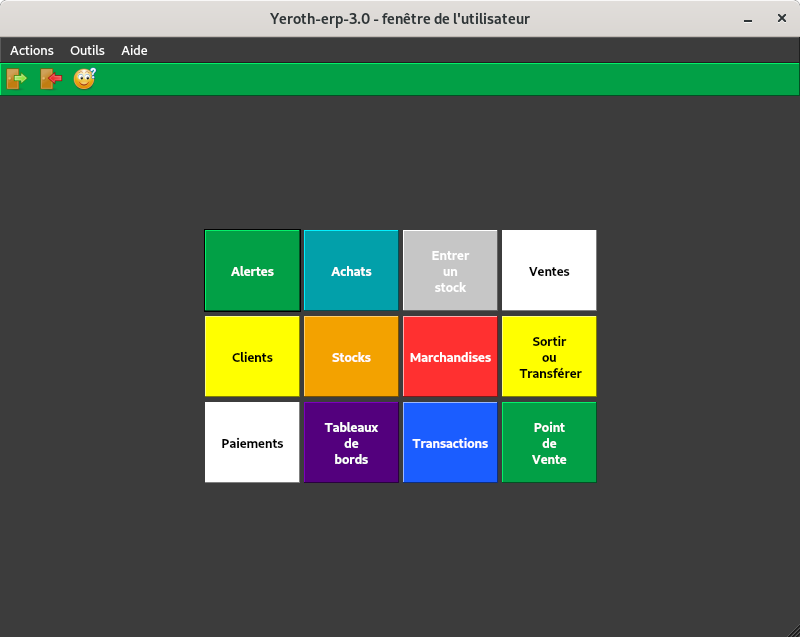
\includegraphics[scale=0.63]{images/yeroth-fenetre-manager.png}
\caption{La fen\^etre d'acceuil d'un \manager}
\label{fig:yeren-fenetre-patron}
\end{figure}

Un utilisateur de \yeren avec le \role \manager a acc\`es
aux fonctionnalit\'es suivantes:
\begin{enumerate}[1)]
	\item administration
	\item alertes
	\item caisse
	\item gestion des achats
	\item gestion des clients
	\item gestion des stocks (voir le Tableau~\ref{tab:taches-fonctions})
	\item tableaux de bords.\\
\end{enumerate}